\documentclass{article}
\usepackage{graphicx} % Required for inserting images
\usepackage[left=1.5cm, right=2cm, top=2cm, bottom=2cm]{geometry}
\usepackage[T1]{fontenc}    %  (ą, ł, ś)
\usepackage[utf8]{inputenc} %  UTF-8
\usepackage[colorlinks=true, linkcolor=black,citecolor=black]{hyperref}
\usepackage[polish]{babel}
\usepackage[polish]{cleveref}
\usepackage{array}
\usepackage{float}
\usepackage{makecell}
\usepackage{multirow}
\usepackage{amsmath}
\usepackage{gensymb}
\usepackage[table]{xcolor}
\documentclass[12pt]{article}
\setlength{\intextsep}{5pt}   
\setlength{\floatsep}{3pt}     
\setlength{\textfloatsep}{5pt} 
\crefname{figure}{Rys.}{Rys.}
\Crefname{figure}{Rys.}{Rys.}
\crefname{section}{Rozd.}{Rozdziały}
\Crefname{section}{Rozd.}{Rozdziały}


\title{
\includegraphics[width=0.5\textwidth]{obrazy/logo-pwr-wm.png}\\[0.2cm] \Huge Sprawozdanie z Fizyki \\[0.2cm] \Huge Ćwiczenie 08}
\author{\Large  t0f1x }
\date{Wrocław, xx.xx.20xx, Grupa nr. }
\begin{document}
\maketitle
\tableofcontents
\newpage
\section{Wstęp}
\label{Wstep}
Ćwiczenie ma na celu badanie ruchu ciał spadających w ośrodku ciekłym, wyznaczenie współczynnika lepkości cieczy metodą Stokesa. Do pomiarów wykorzystane takie środki pomiarowe: Naczynie cylindryczne z badaną cieczą, Areometr, Zestaw kulek, Waga, Mikrometr, Linijka z podziałką milimetrową, Stoper. Kulki zostały oznaczone numerami 1,2,3. Do tabeli zostały wpisane niepewności pomiarowe, podane przez prowadzącego. \\

Podstawą metody Stokesa jest wykorzystanie siły oporu lepkości działającej na ciało o kształcie kuli, poruszające się ruchem jednostajnym w cieczy. Podczas ćwiczenia zmierzono czas opadania kulek na określonej drodze, co pozwoliło na wyznaczenie ich prędkości. Znając gęstość kulek oraz badanej cieczy (wyznaczoną areometrem), na podstawie prawa Stokesa obliczono współczynnik lepkości dynamicznej gliceryny. Zastosowane przyrządy pozwoliły na uwzględnienie błędów systematycznych oraz statystyczną obróbkę wyników pomiarów, co umożliwiło rzetelne określenie niepewności pomiarowej.
\begin{figure}[h]
    \centering
    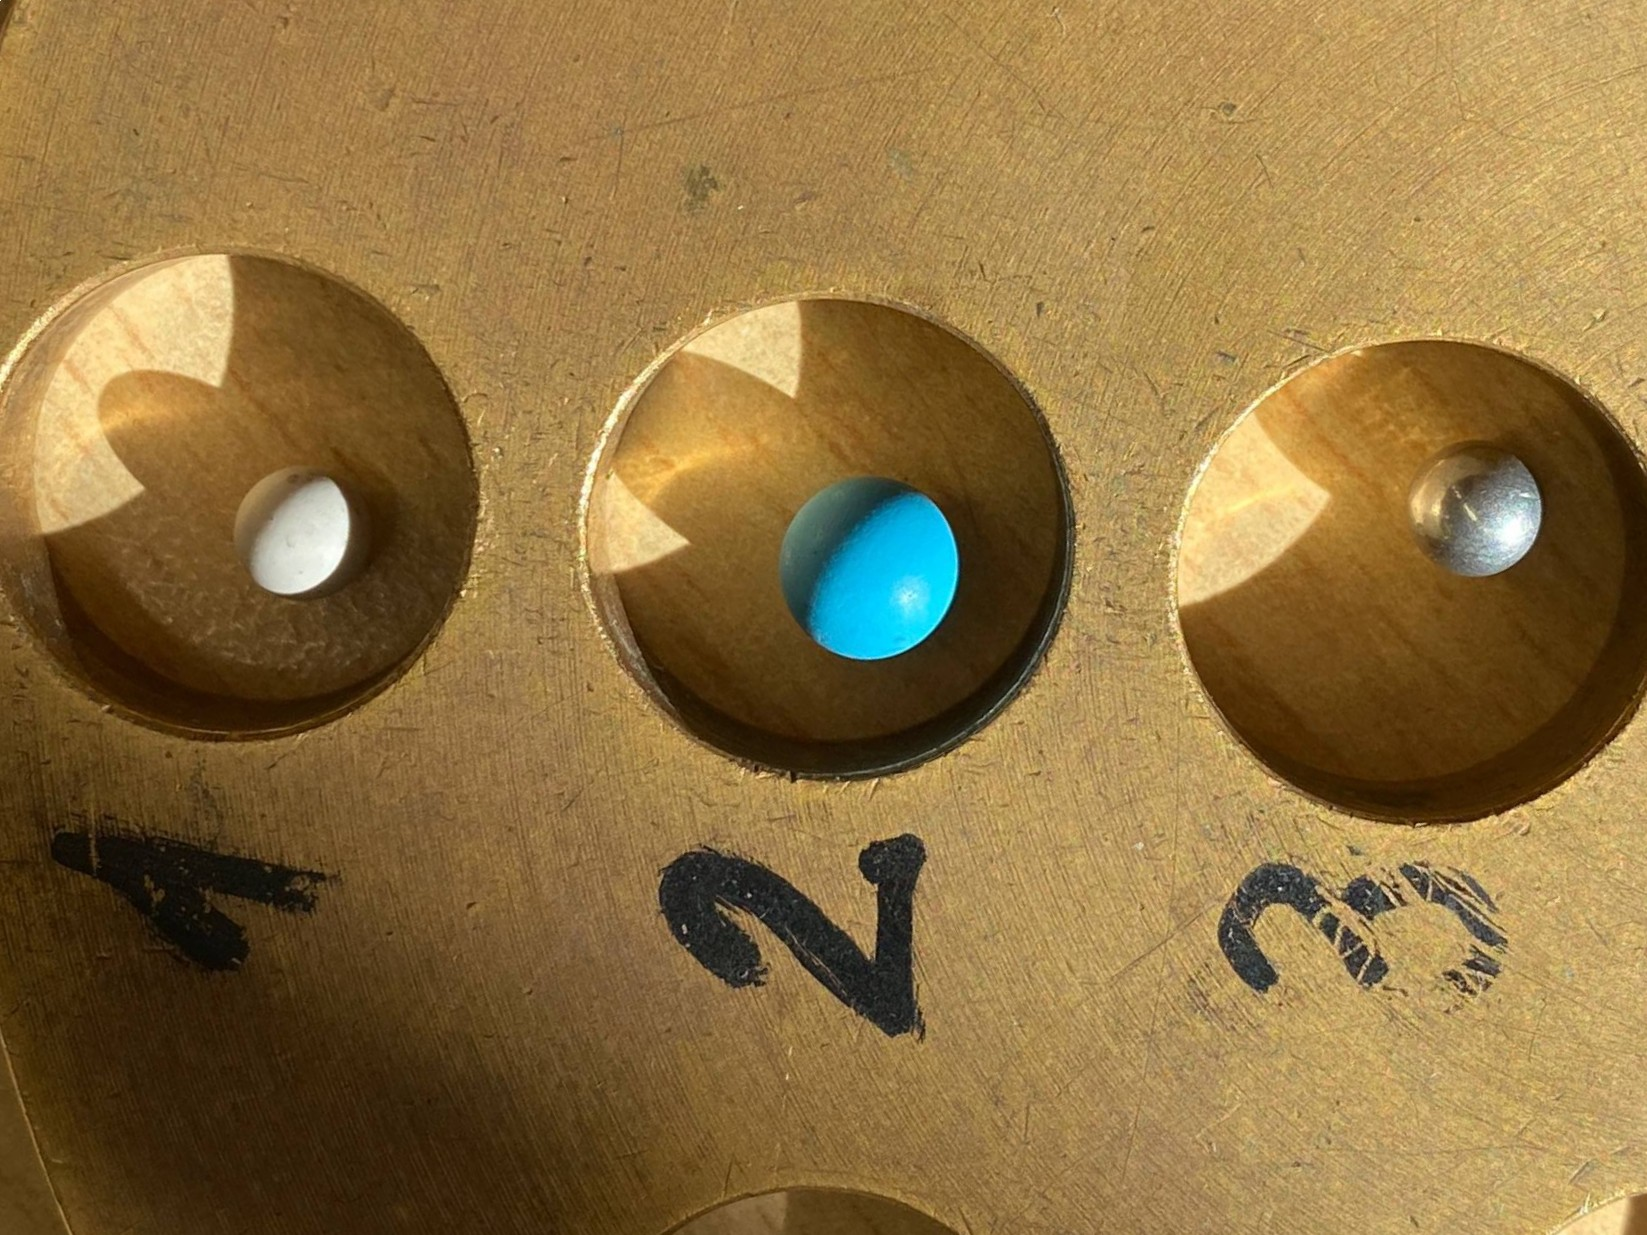
\includegraphics[angle=270, width=0.5\linewidth]{obrazy/ozn kukek.jpg}
    \caption{Przyjęte oznaczenia kulek}
    \label{fig:kulki}
\end{figure}
\\
\begin{table}[h]
    \centering
    \renewcommand{\arraystretch}{1.5}
    \begin{tabular}{|c|c|c|c|c|c|}
    \hline
    Symbol & $u(m)$ [kg] & $u(d)$ [m] & $u(h)$ [m] & $u(\rho)$ [kg/m$^3$] & $u(t)$ [s] \\ \hline
    Wartość & $1 \cdot 10^{-5}$ & $1 \cdot 10^{-5}$ & $1 \cdot 10^{-3}$ & $10$ & $0,4$ \\ \hline
    \end{tabular}
    \caption{Przyjęte niepewności pomiarowe}
    \label{tab:niepewnosci}
\end{table}

\newpage
\section{Wyniki}

\begin{table}[H]
    \centering
    \renewcommand{\arraystretch}{1.2}
    \def\thickline{\noalign{\hrule height 1.5pt}}
    \resizebox{0.75\textwidth }{!}{
        \begin{tabular}{|c|c|c|c|c|c|c|c|c|}
        \hline
        \makecell{Kulka} & \makecell{Lp.} & \makecell{$d \cdot 10^{-3}$ \\ $[m]$} & \makecell{$m \cdot 10^{-3}$ \\ $[kg]$} & \makecell{$t \ [^\circ C]$} & \makecell{$h \cdot 10^{-3}$ \\ $[m]$} & \makecell{$\rho_c$ \\ $[kg/m^3]$} & \makecell{$\rho_k$ \\ $[kg/m^3]$} & \makecell{$\eta$ \\ $[Ns/m^2]$} \\ \hline
        \multirow{5}{*}{1} & 1 & 5,850 & \multirow{5}{*}{0,18} & \multirow{15}{*}{25} & \multirow{15}{*}{320} & \multirow{15}{*}{1250} & \multirow{5}{*}{1712} & \multirow{5}{*}{0,440} \\ \cline{2-3}
                           & 2 & 5,860 &                      &                      &                      &                      &                   &                   \\ \cline{2-3}
                           & 3 & 5,850 &                      &                      &                      &                      &                   &                   \\ \cline{2-3}
                           & 4 & 5,860 &                      &                      &                      &                      &                   &                   \\ \cline{2-3}
                           & 5 & 5,860 &                      &                      &                      &                      &                   &                   \\ \cline{1-4} \cline{8-9}
        \multirow{5}{*}{2} & 1 & 7,920 & \multirow{5}{*}{0,39} &                      &                      &                      & \multirow{5}{*}{1498} & \multirow{5}{*}{0,688} \\ \cline{2-3}
                           & 2 & 7,920 &                      &                      &                      &                      &                   &                   \\ \cline{2-3}
                           & 3 & 7,920 &                      &                      &                      &                      &                   &                   \\ \cline{2-3}
                           & 4 & 7,920 &                      &                      &                      &                      &                   &                   \\ \cline{2-3}
                           & 5 & 7,930 &                      &                      &                      &                      &                   &                   \\ \cline{1-4} \cline{8-9}
        \multirow{5}{*}{3} & 1 & 5,950 & \multirow{5}{*}{0,32} &                      &                      &                      & \multirow{5}{*}{2904} & \multirow{5}{*}{0,625} \\ \cline{2-3}
                           & 2 & 5,940 &                      &                      &                      &                      &                   &                   \\ \cline{2-3}
                           & 3 & 5,950 &                      &                      &                      &                      &                   &                   \\ \cline{2-3}
                           & 4 & 5,950 &                      &                      &                      &                      &                   &                   \\ \cline{2-3}
                           & 5 & 5,950 &                      &                      &                      &                      &                   &                   \\ \thickline
        $\Delta X$ &\makecell{N} &0,01 &0,01 &\cellcolor{gray!30} & 1 &10 &\cellcolor{gray!30} &\cellcolor{gray!30} \\ \hline
        $\multirow{3}{*}{\overline{X}}$ &1 &5,856 &\cellcolor{gray!30} &\cellcolor{gray!30} &\cellcolor{gray!30} &\cellcolor{gray!30} &\cellcolor{gray!30} &\cellcolor{gray!30} \\ \cline{2-3}
        &2 &7,922 &\cellcolor{gray!30} &\cellcolor{gray!30} &\cellcolor{gray!30} &\cellcolor{gray!30} &\cellcolor{gray!30} &\cellcolor{gray!30} \\ \cline{2-3}
        &3 &5,948 &\cellcolor{gray!30} &\cellcolor{gray!30} &\cellcolor{gray!30} &\cellcolor{gray!30} &\cellcolor{gray!30} &\cellcolor{gray!30} \\ \thickline
        
        $\multirow{3}{*}{$u(X)$}$ &1 &0.0063 &\multirow{3}{*}{0,0058} &\cellcolor{gray!30} &\multirow{3}{*}{0,58} &\multirow{3}{*}{5,8} &\cellcolor{gray!30} &\cellcolor{gray!30} \\ \cline{2-3}  
        &2 &0,0061 & &\cellcolor{gray!30} & & &\cellcolor{gray!30} &\cellcolor{gray!30} \\ \cline{2-3}  
        &3 &0,0061 & &\cellcolor{gray!30} & & &\cellcolor{gray!30} &\cellcolor{gray!30} \\ \thickline
        
        $\multirow{3}{*}{$u_c(X)$}$ &1 &\cellcolor{gray!30} &\cellcolor{gray!30} &\cellcolor{gray!30} &\cellcolor{gray!30} &\cellcolor{gray!30} &55,4 &0,0528 \\ \cline{2-2} \cline{8-9} 
        &2 &\cellcolor{gray!30} &\cellcolor{gray!30} &\cellcolor{gray!30} &\cellcolor{gray!30} &\cellcolor{gray!30} &22,5 &0,0652 \\ \cline{2-2} \cline{8-9} 
        &3 &\cellcolor{gray!30} &\cellcolor{gray!30} &\cellcolor{gray!30} &\cellcolor{gray!30} &\cellcolor{gray!30} &53,1  &0,0328 \\ \thickline
    \end{tabular}
    }
    \caption{Wyniki pomiarów}
    \label{tab:wyniki}
\end{table}
\(\overline{\eta}=0,584; \ \ \ u(\overline{\eta})=0,0744 \ [\frac{N\cdot s}{m^2}];\) 
\begin{table}[H]
    \centering
    \renewcommand{\arraystretch}{1.2}
    \def\thickline{\noalign{\hrule height 1.5pt}}
    \resizebox{0.28 \textwidth }{!}{
    \begin{tabular}{|c|c|c|c|c|c|c|}
    \hline
    L.p. & $t_1$ [s] & $t_2$ [s] & $t_3$ [s] \\ \hline
    1 & 16,380 & 25,660 & 6,460 \\ \hline
    2 & 17,360 & 25,450 & 6,460 \\ \hline
    3 & 17,170 & 28,470 & 6,750 \\ \hline
    4 & 16,930 & 25,340 & 6,820 \\ \hline
    5 & 16,010 & 26,200 & 6,040 \\ \hline
    6 & 15,390 & 26,330 & 5,850 \\ \hline
    7 & 16,200 & 24,990 & 5,800 \\ \hline
    8 & 15,800 & 26,120 & 6,450 \\ \hline
    9 & 15,980 & 25,050 & 6,020 \\ \hline
    10 & 16,010 & 26,20 & 6,040 \\ \thickline
    $\Delta X$ &0,40 &0,40 &0,40 \\ \hline
    $\overline{X}$ &16,323 & 25,981&6,269 \\ \hline
    $u(X)$ &0,286 &0,372 &0,258 \\ \hline
    \end{tabular}
    }
    \caption{Wyniki pomiarów czasu}
    \label{tab:wyniki_czasu_pelne}
\end{table}

\newpage
\section{Obliczenia}
        \subsection{\centering Wartości średnie średnicy kulek \ \(\overline{d}\)}
            \begin{flalign*}
                \overline{d_N} = \frac{\sum_{i=1}^{n=5} d_i}{5} &&
            \end{flalign*}
            \begin{flalign*}
                \overline{d_1} = \frac{2 \cdot (5,85) + 3 \cdot (5,86)}{5} = 5,856 \cdot 10^{-3} \ [m] &&
            \end{flalign*}
            
        \subsection{\centering Niepewności pomiarowe średnic kulek \(u(d)\)}
            \subsubsection{Niepewność standardowa typu A}
                \begin{flalign*}
                u_A(d_1) = \sqrt{\sum_{i=1}^{n=5} \frac{(d_{1i}-\overline{d_1})^2)}{n \cdot (n-1)}} = \sqrt{\frac{3(5,860-5,856)^2+2(5,850-5,856)^2}{20}} = 0.002449 \ [mm] = 0.0024 \cdot 10^{-3} \ [m] &&
                \end{flalign*}
            \subsubsection{Niepewność standardowa typu B}
                \begin{flalign*}
                    u_B(d_1)=\sqrt{\frac{\bigtriangleup_p^2(d_1)}{3}}=\frac{0.01}{\sqrt{3}}=0.0057735 \ [mm] = 0.0058\cdot 10^{-3} \ [m] &&
                \end{flalign*}    
            \subsubsection{Niepewność standardowa całkowita}
                \begin{flalign*}
                    u(d_1)= \sqrt{u_A ^2(d_1)+ u_B ^2(d_1)} = \sqrt{(0.002449)^2+(0.0057735)^2}=0.006271 [mm] = 0.0063 \cdot 10^{-3} \ [m] &&
                \end{flalign*}
    %czas
        \subsection{\centering Wartości średnie czasów opadania kulek \ \(\overline{t}\)}
            \begin{flalign*}
                \overline{t_N} = \frac{\sum_{i=1}^{n=10} t_i}{10} &&
            \end{flalign*}
            \begin{flalign*}
                \overline{t_1} = \frac{16,38+17,36+17,17+16,93+16,01+15,39+16,20+15,80+15,98+16,01}{10} = 16.323  \ [s] &&
            \end{flalign*}
            
        \subsection{\centering Niepewności pomiarowe czasów opadania kulek \(u(t)\)}
            \subsubsection{Niepewność standardowa typu A}
                \begin{flalign*}
                u_A(t_1) = \sqrt{\sum_{i=1}^{n=10} \frac{(t_{1i}-\overline{t_1})^2)}{n \cdot (n-1)}} = \sqrt{\frac{2,57201}{90}} = 0,16905 \cdot 10^{-3} \ [m] &&
                \end{flalign*}
            \subsubsection{Niepewność standardowa typu B}
                \begin{flalign*}
                    u_B(t_1)=\sqrt{\frac{\bigtriangleup_p^2(t)}{3}}=\frac{0.4}{\sqrt{3}}= 0,23094 \cdot 10^{-3} \ [m] &&
                \end{flalign*}    
            \subsubsection{Niepewność standardowa całkowita}
                \begin{flalign*}
                    u(t_1)= \sqrt{u_A ^2(t_1)+ u_B ^2(t_1)} = \sqrt{(0,16905)^2+(0,23094)^2}=0,286 \cdot 10^{-3} \ [m] &&
                \end{flalign*}
\newpage
    \subsection{\centering Niepewności pomiarowe mas kulek \(u(m)\)}
        \subsubsection{Niepewność standardowa typu B}
            \begin{flalign*}
                u_B(m)=  \sqrt{\frac{\bigtriangleup_p^2(m)}{3}} = \frac{0.01}{\sqrt{3}}=0.0057735 \ [g] = 0.0058\cdot 10^{-3} \ [kg] &&
            \end{flalign*}
        \subsubsection{Niepewność standardowa całkowita}
            \begin{flalign*}
                u(m)= u_B(m)= 0.0058\cdot 10^{-3} \ [kg] &&
            \end{flalign*}
    
    \subsection{\centering Gęstość kulek \ \(\rho_k\)}
        \begin{flalign*}
           \rho_{k1} = \frac{6m}{\pi \cdot d^3} = \frac{6 \cdot 0,18}{\pi \cdot 5,856^3}= \frac{1,08}{630,878}=0,0017119 \ [g/mm^3]= 1712 \ [kg/m^3] &&
        \end{flalign*}

    \subsection{\centering Niepewności gęstości kulek \(u(\rho_k)\)}
    \begin{flalign*}
           u_{c1}(\rho)=\sqrt{(\frac{6}{\pi \cdot d^3})^2 \cdot u^2(m)+(-\frac{18m}{\pi \cdot d^4})^2 \cdot u^2(d)}= \sqrt{(\frac{6}{\pi \cdot (5,856)^3})^2 \cdot (0,0058)^2 + (- \frac{18 \cdot 0,18}{\pi \cdot (5,856)^4})^2 \cdot(0,0063)^2}= && \\
           5,54 \cdot 10^{-5} \ [g/mm^3] = 55,4\  [kg/m^3] &&
        \end{flalign*}
    \subsection{\centering Niepewność pomiaru gęstości cieczy \(u(\rho_c)\)}
    \subsubsection{Niepewność standardowa typu B}
            \begin{flalign*}
                u_B(\rho_c)=  \sqrt{\frac{\bigtriangleup_p^2(\rho_c)}{3}} = \frac{10}{\sqrt{3}}= 5,8 \ [kg/m^3] &&
            \end{flalign*}
    \subsection{\centering Niepewność pomiaru wysokości \(u(h)\)}
    \subsubsection{Niepewność standardowa typu B}
            \begin{flalign*}
                u_B(h)=  \sqrt{\frac{\bigtriangleup_p^2(h)}{3}} = \frac{1}{\sqrt{3}}= 0,58\cdot 10^{-3} \ [m] &&
            \end{flalign*}
            
    \subsection{\centering Współczynnik lepkości cieczy \(\eta\)}
    \begin{flalign*}
           \eta_1= \frac{d^2\cdot g \cdot t \cdot(\rho_k-\rho_c)}{18h}= \frac{5,856^2 \cdot9,81 \cdot16,323(1712-1250)}{18\cdot 320 } =0,440 \ [\frac{N\cdot s}{m^2}] &&
        \end{flalign*}
    \subsection{\centering Niepewność pomiaru współczynnika lepkości cieczy \(u(\eta)\)}
    \begin{flalign*}
        u_c(\eta)= \epsilon_\eta \cdot \eta_n ; \ \epsilon_\eta=  \sqrt{ \left( 2\frac{u( d)}{d} \right)^2 + \left( \frac{u(t)}{t} \right)^2 + \left( \frac{u(\rho_k - \rho_c)}{\rho_k - \rho_c} \right)^2 + \left( \frac{u(h)}{h} \right)^2 } = \\ \sqrt{ \left( 2\frac{0,0063}{5,856} \right)^2 + \left( \frac{0,286}{16,323} \right)^2 + \left( \frac{55,70}{1712-1250} \right)^2 + \left( \frac{0,58}{320} \right)^2 } =0,12 \\ u_c(\eta_1)=0,12\cdot0,440=0,0528 \ [\frac{N\cdot s}{m^2}]  &&
    \end{flalign*}
    \subsection{\centering Niepewność pomiaru współczynnika lepkości cieczy \(u(\overline{\eta})\)}
    \begin{flalign*}
        u(\overline{\eta})= \sqrt{\sum_{i=1}^{n=3} \frac{(\eta_{i}-\overline{\eta})^2)}{n \cdot (n-1)}} = \sqrt{\frac{0,033233}{6}} = 0,0744 \ [\frac{N\cdot s}{m^2}] &&
    \end{flalign*}

\section{Wnioski}
\label{wnioski}
Podczas ćwiczenia laboratoryjnego były przeprowadzone pomiary różnych wielkości fizycznych: odległość, masa, czas, gęstość. Dzięki obróbce pomiarów była uzyskana wielkość współczynnika lepkości badanej cieczy (gliceryny). \\ \(\eta=0,584 \ \pm 0,149 \ [\frac{N\cdot s}{m^2}]\). Obliczona niepewność pomiarowa świadczy o poprawnym wykonaniu ćwiczenia z dopuszczalną dokładnością zgodnie z warunkami ćwiczenia i metodą Stokesa. \\
Wynik został porównany z danymi w literaturze \cite[s.196]{Tabf}. Przy warunkach wykonania ćwiczenia \(t=25 \degree C\) uzyskana wartość pozostaje w zgodności z tablicą w literaturze. Na podstawie w.w. literatury była porównana zmierzona wartość gęstości gliceryny z wartością w tablicach, określono stężenie procentowe roztworu gliceryny, które wynosi ok. 97 \%.

\vfill
\normalsize
\addcontentsline{toc}{section}{Literatura}
\begin{thebibliography}{9}
    \bibitem{Niepewnosci} 
    Ryszard Poprawski,Włodzimierz Salejda, \textit{Ćwiczenia laboratoryjne z Fizyki, cz. 1}, Oficyna Wydawnicza Politechniki Wrocławskiej, Wrocław 2002.
    \bibitem{Tabf} 
    Tomasz Szymczyk, Stanisław Rabiej, Anna Pielesz, Jan Desselberger, \textit{Tablice matematyczne, fizyczne, chemiczne,  astronomiczne}, Świat Książki, Warszawa 2003.
    
\end{thebibliography}
\end{document}